% In the optional argument of the frame below, i.e. \begin{frame}{Title \hfill logo \hfill UNCC Logo}, add a logo for your section in place of the "figs/topic3White.pdf".  Make sure it has a transparent background, and that it uses white elements to ensure it's visible.

\section{Click2ExTable}
\begin{frame}{Example Multi-Slide Table and Equations\hfill 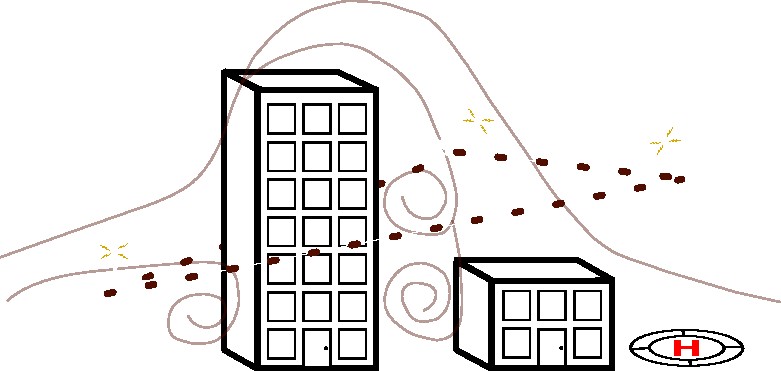
\includegraphics[height=.7cm]{figs/exTopicLogo.pdf} \;\;\;\;\; 
\includegraphics[height=.5cm]{figs/uncc/whiteUNCCLogo.eps}}
    \begin{columns}[T,onlytextwidth]
        \column{0.475\textwidth}
            \only<1-2>{
                In this work, we investigate the use of various feature spaces $F_{i}$ corresponding to respective feature vectors $\bm{x}_i$.  \\ \; \\
                These feature vectors contain some combination of
                \begin{itemize}
                    \item $\bm{r} = $ Locations of wind samples
                    \item $\rho(\bm{r}) , \nabla\rho(\bm{r})= $ SDF and gradient samples at $\bm{r}$
                    \item $\rho(\bm{r}+\bm{b}_{i}) , \nabla\rho(\bm{r}+\bm{b}_{i}) = $ SDF and gradient samples at $\bm{b}_{i}$ points surrounding $\bm{r}$
                \end{itemize}
            }
            \only<3>{
                Some kernels that are investigated with different levels of optimization include:
                \begin{itemize}
                    \item $\kappa_{1}$ - Grouped squared exponential
                        % \vspace{-0.65cm}
                        \begin{align*}
                            \kappa_{1} = &\kappa_{\text{sq}}(\bm{h},\bm{\theta}_{\text{sq},\bm{r}}) + \kappa_{\text{sq}}(\bm{h},\bm{\theta}_{\text{sq},\rho(\bm{r}),\nabla \rho(\bm{r})}) \\ &+ \sum_{i = 1}^{R} \kappa_{\text{sq}}(\bm{h},\bm{\theta}_{\text{sq},\rho(\bm{r}+\bm{b}_{i}),\nabla\rho(\bm{r}+\bm{b}_{i})}) 
                        \end{align*}
                \end{itemize}
            }
            \only<4>{
                Some kernels that are investigated with different levels of optimization include:
                \begin{itemize}
                    \item $\kappa_{1}$ - Grouped squared exponential
                    \item $\kappa_{2}$ - Standard squared exponential $\times$ coregion kernel \cite{bonilla2008, tipping1999}
                \end{itemize}
            }
            \only<5>{
                Some kernels that are investigated with different levels of optimization include:
                \begin{itemize}
                    \item $\kappa_{1}$ - Grouped squared exponential
                    \item $\kappa_{2}$ - Standard squared exponential $\times$ coregion kernel \cite{bonilla2008, tipping1999}
                    \item $\kappa_{3}$ - Standard squared exponential
                        % \vspace{-0.65cm}
                        \begin{align*}  
                            \kappa_{\text{sq}}(\bm{h},\;\bm{\theta}_{\text{sq}}) = \sigma^2 \text{exp}\left(-\frac{1}{2}\sum_{i=1}^{n}\left(\frac{h_i}{L_i}\right)^{2}\right)
                        \end{align*}
                \end{itemize}
            }
        \column{0.475\textwidth}
            \only<1>{
                Candidate vectors include:
                \vspace{-0.7cm}
                \begin{table}[h!]
                \centering
                \resizebox{\textwidth}{!}{%
                \begin{tabular}{ccccccc}
                \hline \hline
                No. & $\bm{r}$ & $\rho(\bm{r})$ & $\nabla \rho(\bm{r})$ & $\rho(\bm{r}+\bm{b}_{i,\dots,B})$ & $\nabla\rho(\bm{r}+\bm{b}_{i,\dots,B})$ \\ \hline
                $F_{1}$ & \cellcolor[HTML]{EFEFEF}\checkmark &  &  &  &   \\
                $F_{2}$ & \cellcolor[HTML]{EFEFEF}\checkmark & \cellcolor[HTML]{EFEFEF}\checkmark & \cellcolor[HTML]{EFEFEF}\checkmark &  &   \\
                $F_{3}$ & \cellcolor[HTML]{EFEFEF}\checkmark & \cellcolor[HTML]{EFEFEF}\checkmark & \cellcolor[HTML]{EFEFEF}\checkmark & \cellcolor[HTML]{EFEFEF}\checkmark & \cellcolor[HTML]{EFEFEF}\checkmark \\
                $F_{4}$ & \cellcolor[HTML]{EFEFEF}\checkmark & \cellcolor[HTML]{EFEFEF}\checkmark & \cellcolor[HTML]{EFEFEF}\checkmark & \cellcolor[HTML]{EFEFEF}\checkmark &   \\
                $F_{5}$ & \cellcolor[HTML]{EFEFEF}\checkmark & \cellcolor[HTML]{EFEFEF}\checkmark &  & \cellcolor[HTML]{EFEFEF}\checkmark &   \\
                $F_{6}$ & \cellcolor[HTML]{EFEFEF}\checkmark & \cellcolor[HTML]{EFEFEF}\checkmark &  &  &   \\
                $F_{7}$ & \cellcolor[HTML]{EFEFEF}\checkmark & \cellcolor[HTML]{EFEFEF}\checkmark & \cellcolor[HTML]{EFEFEF}\checkmark &  & \cellcolor[HTML]{EFEFEF}\checkmark  \\
                $F_{8}$ & \cellcolor[HTML]{EFEFEF}\checkmark &  & \cellcolor[HTML]{EFEFEF}\checkmark &  & \cellcolor[HTML]{EFEFEF}\checkmark  \\ \hline \hline
                \end{tabular}
                }
                \end{table}
            }
            \only<2>{
                Candidate vectors include:
                \vspace{-0.7cm}
                \begin{table}[h!]
                \centering
                \resizebox{\textwidth}{!}{%
                \begin{tabular}{ccccccc}
                \hline \hline
                No. & $\bm{r}$ & $\rho(\bm{r})$ & $\nabla \rho(\bm{r})$ & $\rho(\bm{r}+\bm{b}_{i,\dots,B})$ & $\nabla\rho(\bm{r}+\bm{b}_{i,\dots,B})$ \\ \hline
                $F_{1}$ & \cellcolor[HTML]{EFEFEF}\checkmark &  &  &  &   \\
                $F_{2}$ & \cellcolor[HTML]{EFEFEF}\checkmark & \cellcolor[HTML]{EFEFEF}\checkmark & \cellcolor[HTML]{EFEFEF}\checkmark &  &   \\
                $F_{3}$ & \cellcolor[HTML]{EFEFEF}\checkmark & \cellcolor[HTML]{EFEFEF}\checkmark & \cellcolor[HTML]{EFEFEF}\checkmark & \cellcolor[HTML]{EFEFEF}\checkmark & \cellcolor[HTML]{EFEFEF}\checkmark \\
                $F_{4}$ & \cellcolor[HTML]{EFEFEF}\checkmark & \cellcolor[HTML]{EFEFEF}\checkmark & \cellcolor[HTML]{EFEFEF}\checkmark & \cellcolor[HTML]{EFEFEF}\checkmark &   \\
                $F_{5}$ & \cellcolor[HTML]{EFEFEF}\checkmark & \cellcolor[HTML]{EFEFEF}\checkmark &  & \cellcolor[HTML]{EFEFEF}\checkmark &   \\
                $F_{6}$ & \cellcolor[HTML]{EFEFEF}\checkmark & \cellcolor[HTML]{EFEFEF}\checkmark &  &  &   \\
                $F_{7}$ & \cellcolor[HTML]{EFEFEF}\checkmark & \cellcolor[HTML]{EFEFEF}\checkmark & \cellcolor[HTML]{EFEFEF}\checkmark &  & \cellcolor[HTML]{EFEFEF}\checkmark  \\
                $F_{8}$ & \cellcolor[HTML]{EFEFEF}\checkmark &  & \cellcolor[HTML]{EFEFEF}\checkmark &  & \cellcolor[HTML]{EFEFEF}\checkmark  \\ \hline \hline
                \end{tabular}
                }
                \end{table}
            }
            \only<3>{
                Candidate vectors include:
                \vspace{-0.7cm}
                \begin{table}[h!]
                \centering
                \resizebox{\textwidth}{!}{%
                \begin{tabular}{ccccccc}
                \hline \hline
                No. & $\bm{r}$ & $\rho(\bm{r})$ & $\nabla \rho(\bm{r})$ & $\rho(\bm{r}+\bm{b}_{i,\dots,B})$ & $\nabla\rho(\bm{r}+\bm{b}_{i,\dots,B})$ \\ \hline
                $F_{1}$ & \cellcolor[HTML]{EFEFEF}\checkmark &  &  &  &   \\
                $F_{2}$ & \cellcolor[HTML]{EFEFEF}\checkmark & \cellcolor[HTML]{EFEFEF}\checkmark & \cellcolor[HTML]{EFEFEF}\checkmark &  &   \\
                $F_{3}$ \cellcolor{unccGoldOpaque} & \cellcolor[HTML]{EFEFEF}\checkmark & \cellcolor[HTML]{EFEFEF}\checkmark & \cellcolor[HTML]{EFEFEF}\checkmark & \cellcolor[HTML]{EFEFEF}\checkmark & \cellcolor[HTML]{EFEFEF}\checkmark \\
                $F_{4}$ & \cellcolor[HTML]{EFEFEF}\checkmark & \cellcolor[HTML]{EFEFEF}\checkmark & \cellcolor[HTML]{EFEFEF}\checkmark & \cellcolor[HTML]{EFEFEF}\checkmark &   \\
                $F_{5}$ & \cellcolor[HTML]{EFEFEF}\checkmark & \cellcolor[HTML]{EFEFEF}\checkmark &  & \cellcolor[HTML]{EFEFEF}\checkmark &   \\
                $F_{6}$ & \cellcolor[HTML]{EFEFEF}\checkmark & \cellcolor[HTML]{EFEFEF}\checkmark &  &  &   \\
                $F_{7}$ & \cellcolor[HTML]{EFEFEF}\checkmark & \cellcolor[HTML]{EFEFEF}\checkmark & \cellcolor[HTML]{EFEFEF}\checkmark &  & \cellcolor[HTML]{EFEFEF}\checkmark  \\
                $F_{8}$ & \cellcolor[HTML]{EFEFEF}\checkmark &  & \cellcolor[HTML]{EFEFEF}\checkmark &  & \cellcolor[HTML]{EFEFEF}\checkmark  \\ \hline \hline
                \end{tabular}
                }
                \end{table}
                \textcolor{unccGold}{Gaussian Process Regression (GPR)}\\
                \textcolor{unccClayRed}{Variational GPR (VGP)}
            }
            \only<4>{
                Candidate vectors include:
                \vspace{-0.7cm}
                \begin{table}[h!]
                \centering
                \resizebox{\textwidth}{!}{%
                \begin{tabular}{ccccccc}
                \hline \hline
                No. & $\bm{r}$ & $\rho(\bm{r})$ & $\nabla \rho(\bm{r})$ & $\rho(\bm{r}+\bm{b}_{i,\dots,B})$ & $\nabla\rho(\bm{r}+\bm{b}_{i,\dots,B})$ \\ \hline
                $F_{1}$ \cellcolor{unccclayRedOpaque}& \cellcolor[HTML]{EFEFEF}\checkmark &  &  &  &   \\
                $F_{2}$ & \cellcolor[HTML]{EFEFEF}\checkmark & \cellcolor[HTML]{EFEFEF}\checkmark & \cellcolor[HTML]{EFEFEF}\checkmark &  &   \\
                $F_{3}$ & \cellcolor[HTML]{EFEFEF}\checkmark & \cellcolor[HTML]{EFEFEF}\checkmark & \cellcolor[HTML]{EFEFEF}\checkmark & \cellcolor[HTML]{EFEFEF}\checkmark & \cellcolor[HTML]{EFEFEF}\checkmark \\
                $F_{4}$ & \cellcolor[HTML]{EFEFEF}\checkmark & \cellcolor[HTML]{EFEFEF}\checkmark & \cellcolor[HTML]{EFEFEF}\checkmark & \cellcolor[HTML]{EFEFEF}\checkmark &   \\
                $F_{5}$ & \cellcolor[HTML]{EFEFEF}\checkmark & \cellcolor[HTML]{EFEFEF}\checkmark &  & \cellcolor[HTML]{EFEFEF}\checkmark &   \\
                $F_{6}$ & \cellcolor[HTML]{EFEFEF}\checkmark & \cellcolor[HTML]{EFEFEF}\checkmark &  &  &   \\
                $F_{7}$ & \cellcolor[HTML]{EFEFEF}\checkmark & \cellcolor[HTML]{EFEFEF}\checkmark & \cellcolor[HTML]{EFEFEF}\checkmark &  & \cellcolor[HTML]{EFEFEF}\checkmark  \\
                $F_{8}$ & \cellcolor[HTML]{EFEFEF}\checkmark &  & \cellcolor[HTML]{EFEFEF}\checkmark &  & \cellcolor[HTML]{EFEFEF}\checkmark  \\ \hline \hline
                \end{tabular}
                }
                \end{table}
                \textcolor{unccGold}{Gaussian Process Regression (GPR)}\\
                \textcolor{unccClayRed}{Variational GPR (VGP)}
            }
            \only<5>{
                Candidate vectors include:
                \vspace{-0.7cm}
                \begin{table}[h!]
                \centering
                \resizebox{\textwidth}{!}{%
                \begin{tabular}{ccccccc}
                \hline \hline
                No. & $\bm{r}$ & $\rho(\bm{r})$ & $\nabla \rho(\bm{r})$ & $\rho(\bm{r}+\bm{b}_{i,\dots,B})$ & $\nabla\rho(\bm{r}+\bm{b}_{i,\dots,B})$ \\ \hline
                $F_{1}$ \cellcolor{unccGoldOpaque}& \cellcolor[HTML]{EFEFEF}\checkmark &  &  &  &   \\
                $F_{2}$ \cellcolor{unccGoldOpaque}& \cellcolor[HTML]{EFEFEF}\checkmark & \cellcolor[HTML]{EFEFEF}\checkmark & \cellcolor[HTML]{EFEFEF}\checkmark &  &   \\
                $F_{3}$ \cellcolor{unccGoldOpaque}& \cellcolor[HTML]{EFEFEF}\checkmark & \cellcolor[HTML]{EFEFEF}\checkmark & \cellcolor[HTML]{EFEFEF}\checkmark & \cellcolor[HTML]{EFEFEF}\checkmark & \cellcolor[HTML]{EFEFEF}\checkmark \\
                $F_{4}$ \cellcolor{unccGoldOpaque}& \cellcolor[HTML]{EFEFEF}\checkmark & \cellcolor[HTML]{EFEFEF}\checkmark & \cellcolor[HTML]{EFEFEF}\checkmark & \cellcolor[HTML]{EFEFEF}\checkmark &   \\
                $F_{5}$ \cellcolor{unccGoldOpaque}& \cellcolor[HTML]{EFEFEF}\checkmark & \cellcolor[HTML]{EFEFEF}\checkmark &  & \cellcolor[HTML]{EFEFEF}\checkmark &   \\
                $F_{6}$ \cellcolor{unccGoldOpaque}& \cellcolor[HTML]{EFEFEF}\checkmark & \cellcolor[HTML]{EFEFEF}\checkmark &  &  &   \\
                $F_{7}$ \cellcolor{unccGoldOpaque}& \cellcolor[HTML]{EFEFEF}\checkmark & \cellcolor[HTML]{EFEFEF}\checkmark & \cellcolor[HTML]{EFEFEF}\checkmark &  & \cellcolor[HTML]{EFEFEF}\checkmark  \\
                $F_{8}$ \cellcolor{unccGoldOpaque}& \cellcolor[HTML]{EFEFEF}\checkmark &  & \cellcolor[HTML]{EFEFEF}\checkmark &  & \cellcolor[HTML]{EFEFEF}\checkmark  \\ \hline \hline
                \end{tabular}
                }
                \end{table}
                \textcolor{unccGold}{Gaussian Process Regression (GPR)}\\
                \textcolor{unccClayRed}{Variational GPR (VGP)}
            }
    \end{columns}
    
\end{frame}